% !TEX program = xelatex
% Why Linear Regression — a tutorial
% Author: 熊昊一 (Haoyi Xiong)
\documentclass[11pt, a4paper]{ctexart}

% ---------- Encoding & fonts ----------
\usepackage{xeCJK}
\setCJKmainfont{PingFang SC}  % macOS built-in; fallback: STSong / Source Han Serif
\usepackage{amsmath, amssymb, amsthm, mathtools}
\usepackage{bm}
\usepackage{geometry}
\geometry{margin=2.5cm}

% ---------- Typography ----------
\usepackage{microtype}
\usepackage{enumitem}
\usepackage{booktabs}
\usepackage{xcolor}
\definecolor{accent}{RGB}{0, 90, 160}
\definecolor{lightband}{RGB}{240, 244, 248}
\usepackage{tcolorbox}
\tcbuselibrary{breakable, skins}
\usepackage{graphicx}
\usepackage{tikz}
\usetikzlibrary{arrows.meta, calc, positioning, decorations.pathreplacing}
\usepackage{hyperref}
\hypersetup{
  colorlinks=true,
  linkcolor=accent,
  citecolor=accent,
  urlcolor=accent,
  pdftitle={Why Linear Regression},
  pdfauthor={Haoyi Xiong},
}

% ---------- Theorem-like environments ----------
\theoremstyle{plain}
\newtheorem{theorem}{Theorem}[section]
\newtheorem{lemma}[theorem]{Lemma}
\newtheorem{corollary}[theorem]{Corollary}
\theoremstyle{definition}
\newtheorem{definition}[theorem]{Definition}
\newtheorem{example}[theorem]{Example}
\newtheorem{exercise}{Exercise}[section]
\theoremstyle{remark}
\newtheorem*{remark}{Remark}
\newtheorem*{intuition}{Intuition}

% ---------- Boxes ----------
\newtcolorbox{keybox}[1][]{
  colback=lightband, colframe=accent, fonttitle=\bfseries,
  title={#1}, breakable, sharp corners, boxrule=0.6pt, left=2mm, right=2mm, top=1.5mm, bottom=1.5mm
}

% ---------- Macros ----------
\newcommand{\R}{\mathbb{R}}
\newcommand{\E}{\mathbb{E}}
\newcommand{\Var}{\mathrm{Var}}
\newcommand{\Cov}{\mathrm{Cov}}
\newcommand{\bias}{\mathrm{bias}}
\newcommand{\MSE}{\mathrm{MSE}}
\newcommand{\rank}{\mathrm{rank}}
\newcommand{\trace}{\mathrm{tr}}
\newcommand{\X}{\mathbf{X}}
\newcommand{\y}{\mathbf{y}}
\newcommand{\bhat}{\hat{\bm{\beta}}}
\newcommand{\bbeta}{\bm{\beta}}
\newcommand{\x}{\mathbf{x}}
\newcommand{\zero}{\mathbf{0}}
\newcommand{\norm}[1]{\left\lVert #1 \right\rVert}

\title{\Huge \textbf{Why Linear Regression}\\[4pt]
\Large A First Principles Tutorial}
\author{熊昊一 (Haoyi Xiong)}
\date{\today}

\begin{document}

\maketitle

\begin{abstract}
\noindent
Linear regression is the first model almost everyone learns and the model almost everyone underestimates.
This tutorial is not about \emph{how} to run \texttt{lm()} in R or \texttt{LinearRegression()} in scikit-learn — it is about \emph{why} the method works, why squared error, why the normal equations, and why, after two centuries, a straight line is still where honest data analysis begins.
We derive everything from first principles: the calculus of least squares, the geometry of projections, the Gauss--Markov theorem, the probabilistic view through maximum likelihood, and the modern view through bias--variance trade-off and regularization.
Only high-school calculus and basic linear algebra are assumed.
\end{abstract}

\newpage
\tableofcontents
\newpage

% Chapter 1
\section{Introduction: The Most Important Model You Will Ever Learn}\label{sec:intro}

\subsection{The question this tutorial answers}

Every machine-learning course, every statistics textbook, and every data-science bootcamp introduces linear regression within the first two weeks. And almost all of them do it backwards: they hand you a formula,
\[
  \hat{\beta} = (\X^\top \X)^{-1} \X^\top \y,
\]
tell you to trust it, and move on to ``more exciting'' models.

This tutorial goes the other way. We will earn every step. By the end you will be able to answer, from first principles:

\begin{enumerate}[label=(\arabic*)]
  \item Why do we fit a \emph{line} (or hyperplane) at all? What is the underlying assumption, and how strong is it?
  \item Why \emph{squared} error? Why not absolute error, or error to the fourth power?
  \item Where does the magic formula $\hat{\beta} = (\X^\top\X)^{-1}\X^\top\y$ come from, and what does it mean geometrically?
  \item Under what conditions is the ordinary least squares (OLS) estimator the \emph{best} estimator? (Answer: the Gauss--Markov theorem.)
  \item What do we gain — and what do we quietly assume — when we view regression through probability (maximum likelihood)?
  \item Why does adding a penalty term (ridge, lasso) help, and what does the bias--variance trade-off have to do with it?
  \item Why does a 200-year-old linear method still sit underneath logistic regression, neural networks, and half of modern statistics?
\end{enumerate}

\subsection{A 200-year-old idea that refuses to die}

Least squares was published independently by Legendre (1805) and Gauss (1809), who used it to predict the orbit of the asteroid Ceres from noisy astronomical observations. The method has survived every paradigm shift since: the computer, the bootstrap, the deep-learning revolution. There is a reason.

\begin{keybox}[Thesis of this tutorial]
Linear regression is not popular because real-world relationships are linear. They rarely are. It is popular because
\begin{enumerate}[label=(\roman*)]
  \item a local linear approximation is often good enough (Taylor's theorem);
  \item it is the \emph{uniquely solvable, uniquely interpretable, uniquely honest} baseline — everything else is measured against it;
  \item it is the exact foundation on which logistic regression, generalized linear models, kernel methods, and even neural networks are built.
\end{enumerate}
\end{keybox}

\subsection{What you need to know before starting}

\begin{itemize}
  \item \textbf{Calculus}: partial derivatives, the chain rule, and the fact that a minimum of a smooth function occurs where its derivative is zero.
  \item \textbf{Linear algebra}: vectors, matrices, matrix multiplication, transpose, inverse; matrix-vector products as linear combinations. Appendix~\ref{app:linalg} collects everything we use.
  \item \textbf{Probability} (helpful, not required until Chapter~\ref{sec:probability}): expectation, variance, the Gaussian distribution.
\end{itemize}

Everything else is derived here.

\subsection{The setup, stated once and for all}

We are given $n$ observations. Each observation $i$ consists of a \emph{response} (target, dependent variable) $y_i \in \R$ and $p$ \emph{features} (predictors, covariates, independent variables) $x_{i1}, \dots, x_{ip} \in \R$. We believe the responses were generated as
\begin{equation}\label{eq:model}
  y_i = \beta_0 + \beta_1 x_{i1} + \beta_2 x_{i2} + \dots + \beta_p x_{ip} + \varepsilon_i,
  \qquad i = 1, \dots, n,
\end{equation}
where $\beta_0, \dots, \beta_p$ are unknown constants we want to estimate, and $\varepsilon_i$ is an \emph{error term} capturing everything the line misses: measurement noise, omitted variables, genuine randomness, and the sin of approximating a nonlinear world with a hyperplane.

In matrix form, with $\X \in \R^{n \times (p+1)}$ the design matrix whose $i$-th row is $(1, x_{i1}, \dots, x_{ip})$, $\bbeta \in \R^{p+1}$ the parameter vector, and $\bm{\varepsilon} \in \R^n$ the errors:
\begin{equation}\label{eq:model-matrix}
  \y = \X \bbeta + \bm{\varepsilon}.
\end{equation}

The whole game of this tutorial is understanding what the words ``linear'' and ``error'' really commit us to, and what the best possible estimate of $\bbeta$ is under each interpretation.

\begin{remark}[Linear in \emph{what}?]
``Linear'' in \emph{linear regression} means linear in the \emph{parameters} $\beta_j$, not necessarily linear in the raw features. The model $y = \beta_0 + \beta_1 x + \beta_2 x^2 + \beta_3 \sin x + \varepsilon$ is perfectly linear by our definition: define the new features $\tilde{x}_1 = x$, $\tilde{x}_2 = x^2$, $\tilde{x}_3 = \sin x$ and it has the form of \eqref{eq:model}. What is \emph{not} linear is $y = \beta_0 + e^{\beta_1 x} + \varepsilon$. This flexibility — turning nonlinear relationships into linear ones by feature engineering — is a recurring theme (Chapter~\ref{sec:beyond}).
\end{remark}

% Chapter 2
\section{Least Squares: Deriving the Estimator from Scratch}\label{sec:ls}

\subsection{The problem as an optimization problem}

Forget statistics for a moment. We have $n$ points and we want a line (hyperplane) that passes ``as close as possible'' to all of them. ``Close'' must be made precise, and the most natural first guess — the one Legendre and Gauss made — is to measure total misfit by the \emph{sum of squared residuals}:
\begin{equation}\label{eq:rss}
  S(\bbeta) = \sum_{i=1}^{n} \big( y_i - \beta_0 - \beta_1 x_{i1} - \dots - \beta_p x_{ip} \big)^2
            = \norm{\y - \X \bbeta}^2.
\end{equation}
Each term $e_i = y_i - (\X \bbeta)_i$ is the \emph{residual}: the vertical gap between the observation and the fitted hyperplane. Squaring does three useful things at once: it makes every deviation positive, it penalizes large deviations disproportionately, and — crucially, as we will see — it makes the problem \emph{differentiable and convex}, hence exactly solvable. Chapter~\ref{sec:why-squared} interrogates whether this is the ``right'' loss; for now we simply adopt it.

The \textbf{ordinary least squares (OLS) estimator} is
\[
  \bhat \;=\; \arg\min_{\bbeta \in \R^{p+1}} \; \norm{\y - \X \bbeta}^2.
\]

\subsection{The one-variable warm-up: $p = 0$ and $p = 1$}

\textbf{No features ($p=0$): only an intercept.} Minimize $S(\beta_0) = \sum_i (y_i - \beta_0)^2$. Setting the derivative to zero:
\[
  \frac{dS}{d\beta_0} = -2 \sum_{i=1}^n (y_i - \beta_0) = 0
  \quad\Longrightarrow\quad
  \hat{\beta}_0 = \frac{1}{n} \sum_{i=1}^n y_i = \bar{y}.
\]
The least-squares fit with no features is just the mean. Already a theorem is visible: \emph{least squares generalizes the average}. The sample mean is the value that minimizes squared deviation — a fact we will reuse constantly.

\textbf{One feature ($p=1$): the regression line through a scatter plot.} Minimize
\[
  S(\beta_0, \beta_1) = \sum_{i=1}^n (y_i - \beta_0 - \beta_1 x_i)^2.
\]
Take partial derivatives and set them to zero (the ``normal equations'' in disguise):
\[
  \frac{\partial S}{\partial \beta_0} = -2 \sum_i (y_i - \beta_0 - \beta_1 x_i) = 0,
  \qquad
  \frac{\partial S}{\partial \beta_1} = -2 \sum_i x_i (y_i - \beta_0 - \beta_1 x_i) = 0.
\]
From the first equation, $\hat{\beta}_0 = \bar{y} - \hat{\beta}_1 \bar{x}$: the line passes through the centroid $(\bar{x}, \bar{y})$ of the data. Substituting into the second equation and solving:
\begin{equation}\label{eq:slope}
  \hat{\beta}_1 = \frac{\sum_i (x_i - \bar{x})(y_i - \bar{y})}{\sum_i (x_i - \bar{x})^2} = \frac{\Cov_n(x, y)}{\Var_n(x)},
\end{equation}
where $\Cov_n, \Var_n$ denote the sample (dividing by $n$ or $n-1$ — the ratio is the same) covariance and variance.

Read \eqref{eq:slope} slowly: \emph{the slope is the ratio of how $x$ and $y$ vary together to how much $x$ varies alone}. This is the single most quoted formula in applied statistics, and it has fallen out of nothing more than setting a derivative to zero. Nothing in it assumed the errors were Gaussian, independent, or even random — the least-squares machinery is purely geometric optimization.

\begin{example}[Computation by hand]\label{ex:hand}
Take $n = 4$ points $(x, y) = (1, 2), (2, 3), (3, 5), (4, 4)$. Then $\bar{x} = 2.5$, $\bar{y} = 3.5$,
$\sum_i (x_i - \bar{x})(y_i - \bar{y}) = (-1.5)(-1.5) + (-0.5)(-0.5) + (0.5)(1.5) + (1.5)(0.5) = 4$, and $\sum_i (x_i - \bar{x})^2 = 2.25 + 0.25 + 0.25 + 2.25 = 5$, so $\hat{\beta}_1 = 4/5 = 0.8$ and $\hat{\beta}_0 = 3.5 - 0.8 \times 2.5 = 1.5$. The least-squares line is $y = 1.5 + 0.8x$. You can verify the normal equations directly: residuals $e_i = y_i - \hat{y}_i = (2 - 2.3,\; 3 - 3.1,\; 5 - 3.9,\; 4 - 4.7) = (-0.3, -0.1, 1.1, -0.7)$ sum to $0$, and $\sum_i x_i e_i = -0.3 - 0.2 + 3.3 - 2.8 = 0$ — residual orthogonal to the design, as promised.
\end{example}

\subsection{The general case: the normal equations}

Now let $\X \in \R^{n \times (p+1)}$ with $n > p+1$. Expand the objective:
\[
  S(\bbeta) = (\y - \X\bbeta)^\top (\y - \X\bbeta)
            = \y^\top \y - 2 \bbeta^\top \X^\top \y + \bbeta^\top \X^\top \X \bbeta,
\]
using $\y^\top \X \bbeta = \bbeta^\top \X^\top \y$ (both are scalars). Differentiate with respect to the vector $\bbeta$ — using the two elementary identities $\nabla_{\bbeta}(\bm{c}^\top \bbeta) = \bm{c}$ and $\nabla_{\bbeta}(\bbeta^\top \bm{A} \bbeta) = 2 \bm{A} \bbeta$ for symmetric $\bm{A}$:
\begin{equation}\label{eq:grad}
  \nabla_{\bbeta} S = -2 \X^\top \y + 2 \X^\top \X \bbeta.
\end{equation}
Setting the gradient to zero yields the \textbf{normal equations}:
\begin{equation}\label{eq:normal}
  \boxed{\;\X^\top \X \, \bhat \;=\; \X^\top \y\;}
\end{equation}

Provided $\X$ has full column rank (i.e., $\rank(\X) = p+1$, no feature is a linear combination of the others, and $n \geq p+1$), the Gram matrix $\X^\top \X$ is symmetric positive definite hence invertible, and we obtain the celebrated closed form
\begin{equation}\label{eq:ols}
  \boxed{\;\bhat = (\X^\top \X)^{-1} \X^\top \y.\;}
\end{equation}

\begin{remark}[Why ``normal''?]
The equations \eqref{eq:normal} say $\X^\top (\y - \X \bhat) = \zero$: the residual vector is \emph{orthogonal} (normal, in the geometric sense) to every column of $\X$. This is not a coincidence or a curiosity — it is the entire geometric content of least squares, and Chapter~\ref{sec:geometry} is devoted to it.
\end{remark}

\begin{remark}[Why is it a minimum?]
The Hessian $\nabla^2 S = 2 \X^\top \X$ is positive definite when $\X$ has full column rank, so $S$ is strictly convex and the stationary point is the \emph{unique global minimum}. There are no spurious local minima, no initialization issues, no learning rates. Compare that with training a neural network. This exactness is a large part of ``why linear regression.''
\end{remark}

\subsection{Rank deficiency and the pseudoinverse}

What if $\X^\top \X$ is singular — some feature is redundant, or $p \geq n$? The minimizer is no longer unique (a whole flat subspace of $\bbeta$'s attains the minimum), but the \emph{fitted values} $\X \bhat$ still are. The canonical choice is the \textbf{Moore--Penrose pseudoinverse} solution
\[
  \bhat = \X^{+} \y,
\]
which picks, among all minimizers, the one with smallest Euclidean norm. Every serious implementation (R's \texttt{lm}, NumPy's \texttt{lstsq}, scikit-learn's \texttt{LinearRegression}) computes exactly this via the SVD or QR decomposition rather than forming $(\X^\top\X)^{-1}$, for numerical stability. This foreshadows Chapter~\ref{sec:bias-variance}: with redundant or numerous features, constraining the solution norm is not merely a numerical trick, it is a statistical idea (ridge regression).

\subsection{Fitted values, residuals, and $R^2$}

Given $\bhat$, define the \textbf{fitted values} $\hat{\y} = \X \bhat$ and \textbf{residuals} $\bm{e} = \y - \hat{\y}$. Two facts follow immediately from the normal equations:

\begin{enumerate}[label=(\alph*)]
  \item $\X^\top \bm{e} = \zero$: residuals are orthogonal to every column of $\X$. In particular, with an intercept column, $\sum_i e_i = 0$: residuals average to zero.
  \item $\hat{\y}^\top \bm{e} = (\X \bhat)^\top \bm{e} = \bhat^\top \X^\top \bm{e} = 0$: fitted values and residuals are orthogonal.
\end{enumerate}

Fact (b) yields the \textbf{Pythagorean decomposition} (with an intercept):
\[
  \norm{\y - \bar{y} \mathbf{1}}^2
  = \norm{\hat{\y} - \bar{y} \mathbf{1}}^2 + \norm{\bm{e}}^2,
\]
i.e., \emph{total variation = explained variation + unexplained variation}. Dividing through:
\begin{equation}\label{eq:r2}
  R^2 = 1 - \frac{\sum_i e_i^2}{\sum_i (y_i - \bar{y})^2}
      = \frac{\norm{\hat{\y} - \bar{y}\mathbf{1}}^2}{\norm{\y - \bar{y}\mathbf{1}}^2} \in [0, 1].
\end{equation}
$R^2$ is the fraction of variance ``explained'' by the regression, and it is literally the squared cosine of the angle between $\y - \bar{y}\mathbf{1}$ and its projection onto the column space — geometry again.

\begin{keybox}[What we have established so far]
Without a single probabilistic assumption:
\begin{itemize}
  \item the least-squares estimator has the closed form $\bhat = (\X^\top \X)^{-1} \X^\top \y$ (unique iff $\X$ has full column rank);
  \item it is the unique global minimizer (convexity);
  \item residuals are orthogonal to the design matrix (the normal equations);
  \item $R^2$ decomposes variance via the Pythagorean theorem.
\end{itemize}
Everything so far is \emph{deterministic geometry}. Statistics enters when we ask how good $\bhat$ is \emph{as an estimate of the truth} — that is the business of Chapters \ref{sec:gauss-markov} and \ref{sec:probability}.
\end{keybox}

% Chapter 3
\section{Why Squared Error? Interrogating the Loss Function}\label{sec:why-squared}

We minimized the sum of squared residuals because Legendre and Gauss did. But 220 years later we are allowed to ask: was that the right choice? This chapter compares the leading candidates and extracts the deep reasons squared error keeps winning.

\subsection{The candidate losses}

For a residual $e$, consider the penalty $\rho(e)$:

\begin{center}
\begin{tabular}{@{}llll@{}}
\toprule
Loss & $\rho(e)$ & Estimator it yields (location problem) & Behaviour \\
\midrule
Squared & $e^2$ & mean & smooth, strongly convex \\
Absolute & $|e|$ & median & robust, piecewise linear \\
$0/1$-ish & $\mathbb{1}\{|e| > \delta\}$ & mode / majority & discontinuous, combinatorial \\
Huber & $\begin{cases} \frac{1}{2}e^2 & |e|\le\delta \\ \delta|e| - \frac{1}{2}\delta^2 & |e| > \delta\end{cases}$ & between mean and median & smooth + robust \\
Quartic & $e^4$ & \emph{not robust at all} & over-penalizes outliers \\
\bottomrule
\end{tabular}
\end{center}

Minimizing $\sum_i |y_i - \theta|$ over $\theta$ yields the \emph{sample median}; minimizing $\sum_i (y_i - \theta)^2$ yields the \emph{mean}. So the choice of loss \emph{is} the choice of which notion of ``center'' the model pursues. Why prefer the mean's sensitivity over the median's robustness? Three answers.

\subsection{Answer 1: differentiability and exact solvability}

$e^2$ is smooth and strictly convex; $|e|$ is not differentiable at $0$ and only piecewise linear. Consequences:

\begin{itemize}
  \item With squared loss, setting the gradient to zero gives the \emph{linear} normal equations \eqref{eq:normal} — solvable in one shot, unique minimizer, no algorithmic subtleties.
  \item With absolute loss, the optimum satisfies a \emph{set of inequalities} (a median condition) and must be found by linear programming or iteratively reweighted least squares. For a century and a half — no computers — this alone settled the argument.
\end{itemize}

Modern computation softens this argument (median regression is now routine), but it does not erase it: the entire inferential apparatus of regression (standard errors, $t$-tests, $F$-tests, confidence ellipsoids) is built on the quadratic geometry of squared loss. Change the loss and you rebuild statistics from scratch — which is a respectable thing to do, but it is a different tutorial.

\subsection{Answer 2: maximum likelihood under Gaussian noise}\label{sec:why-squared-mle}

Here is the probabilistic argument, due to Gauss (1809) — who inverted it, deriving the Gaussian density \emph{from} the requirement that least squares be optimal. Suppose the errors in \eqref{eq:model-matrix} are independent with $\varepsilon_i \sim \mathcal{N}(0, \sigma^2)$. Then the likelihood of observing $\y$ given $\bbeta$ is
\[
  L(\bbeta) = \prod_{i=1}^n \frac{1}{\sqrt{2\pi}\sigma} \exp\!\left( -\frac{(y_i - \x_i^\top \bbeta)^2}{2\sigma^2} \right).
\]
The log-likelihood is
\[
  \ell(\bbeta) = \text{const} - \frac{1}{2\sigma^2} \sum_{i=1}^n (y_i - \x_i^\top \bbeta)^2.
\]
Maximizing $\ell$ over $\bbeta$ is \emph{identical} to minimizing the sum of squared residuals. In one line:
\[
  \boxed{\;\text{OLS} = \text{MLE under i.i.d.\ Gaussian errors}.\;}
\]
The Gaussian assumption, in turn, is not arbitrary: by the central limit theorem, errors that are the sum of many small independent disturbances tend to be Gaussian; and the Gaussian is the maximum-entropy distribution with fixed variance — the ``least informative'' error model consistent with a given noise level.

Note the asymmetry in what this proves: squared loss is optimal \emph{if} errors are Gaussian, and badly suboptimal if errors are heavy-tailed (Chapter~\ref{sec:practice}). The mean chases outliers; the median shrugs at them. This is the honest, complete answer to ``why squared'': it is the right loss for a specific, defensible noise model, and a fragile one outside it.

\subsection{Answer 3: Gauss's counterfactual — deriving the Gaussian from least squares}

Gauss asked the reverse question: \emph{what error distribution makes the sample mean (the least-squares estimate of location) equal to the maximum likelihood estimate?} The answer, up to location and scale, is the Gaussian density
\[
  \varphi(x) = \frac{1}{\sqrt{2\pi}\sigma} e^{-x^2 / 2\sigma^2}.
\]
Sketch: in the location problem $y_i = \mu + \varepsilon_i$, MLE sets $\sum_i \frac{\varphi'}{\varphi}(y_i - \mu) = 0$. For this to hold at $\mu = \bar{y}$ for \emph{every} sample, one needs $\frac{\varphi'}{\varphi}$ linear, i.e.\ $\varphi'/\varphi(x) = -x/\sigma^2$, whose solution is the Gaussian. So the Gaussian density and the squared loss are \emph{matched pairings} — each is the natural partner of the other. This mutual optimality, not coincidence, is the deepest ``why squared'' there is.

\subsection{What squared error quietly assumes — and the modern repair}

Squaring penalizes large errors \emph{quadratically}, so a single corrupted point with residual $10$ is penalized $100$ times as much as one with residual $1$; a residual of $100$, $10{,}000$ times. OLS is therefore \emph{non-robust}: a few gross outliers can drag the fitted line arbitrarily far. Practitioners have two honest responses:

\begin{enumerate}[label=(\roman*)]
  \item \textbf{Diagnose}: plot residuals; if the few large ones are data errors, fix or remove them (Chapter~\ref{sec:practice}).
  \item \textbf{Change the loss}: Huber's loss behaves like $e^2$ near zero (efficient for Gaussian-like bulk) and like $|e|$ in the tails (bounded influence of outliers). Its estimator is computed by iteratively reweighted least squares — literally running OLS over and over with weights that downweight large residuals, a beautiful case of the classical method \emph{inside} the modern repair.
\end{enumerate}

\begin{keybox}[Verdict on squared error]
Squared error is not a law of nature; it is the optimal loss under Gaussian noise, the uniquely tractable smooth loss, and half of a matched pair with the Gaussian distribution. Use it by default, know what it costs (sensitivity to outliers), and know the repair (robust losses, diagnostics). Knowing \emph{when} your default breaks is the real lesson of this chapter.
\end{keybox}

% Chapter 4
\section{The Geometry of Least Squares: Regression as Projection}\label{sec:geometry}

Statistics courses present $\bhat = (\X^\top \X)^{-1} \X^\top \y$ as a formula to memorize. This chapter shows that the formula \emph{is} a picture: fitting a linear model is projecting the response vector onto the column space of the design matrix. Once you see the picture, the normal equations, $R^2$, the hat matrix, and even multicollinearity become obvious.

\subsection{Column space and the projection problem}

Let $\X = [\x_0, \x_1, \dots, \x_p] \in \R^{n \times (p+1)}$ with columns $\x_j \in \R^n$. The \textbf{column space} (or \emph{range})
\[
  \mathcal{C}(\X) = \{ \X \bbeta : \bbeta \in \R^{p+1} \} \subseteq \R^n
\]
is the set of all vectors the model can possibly produce — the set of all fitted-value vectors. It is a linear subspace of dimension $\rank(\X) = p+1$ (assuming full rank).

Fitting the model means: \emph{find the point of $\mathcal{C}(\X)$ closest to $\y$}. The Euclidean distance from $\y$ to $\X\bbeta$ is exactly $\norm{\y - \X\bbeta}$ — the square root of our loss \eqref{eq:rss}. So:

\begin{keybox}[The geometric statement of least squares]
\[
  \bhat = \arg\min_{\bbeta} \norm{\y - \X \bbeta}
  \quad\Longleftrightarrow\quad
  \X \bhat \text{ is the orthogonal projection of } \y \text{ onto } \mathcal{C}(\X).
\]
OLS is the closest the model's subspace can come to the data. Nothing more, nothing less.
\end{keybox}

\subsection{Why the normal equations are the Pythagorean theorem}

Take any candidate $\X \bbeta \in \mathcal{C}(\X)$. Decompose $\y = \X\bhat + \bm{e}$. The normal equations say $\X^\top \bm{e} = 0$, i.e.\ $\bm{e} \perp \mathcal{C}(\X)$. For any other point $\X \bbeta$ in the subspace, the vector $\X(\bbeta - \bhat)$ lies in $\mathcal{C}(\X)$, hence is orthogonal to $\bm{e}$. By Pythagoras:
\[
  \norm{\y - \X \bbeta}^2
  = \norm{\X(\bhat - \bbeta) + \bm{e}}^2
  = \norm{\X(\bhat - \bbeta)}^2 + \norm{\bm{e}}^2
  \;\geq\; \norm{\bm{e}}^2 = \norm{\y - \X \bhat}^2,
\]
with equality iff $\bbeta = \bhat$. This is a \emph{proof without calculus}: orthogonality implies optimality, and conversely, any optimal point must have residual orthogonal to the subspace (otherwise you could slide along the subspace to get closer). The normal equations are not an algebraic accident — they are the statement that the residual is perpendicular to the model's world.

\begin{figure}[htbp]
\centering
\resizebox{0.88\linewidth}{!}{%
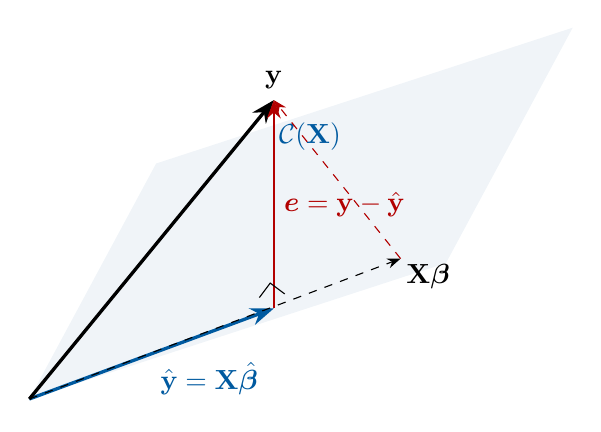
\begin{tikzpicture}[scale=1.15, >=Stealth]
  % column space plane
  \coordinate (O) at (0,0);
  \coordinate (u) at (4.6,1.5);
  \coordinate (v) at (1.4,2.6);
  \fill[lightband] (O) -- (u) -- ($(u)+(v)$) -- (v) -- cycle;
  \node[color=accent] at (3.1,2.9) {$\mathcal{C}(\X)$};
  % vectors
  \coordinate (yhat) at (2.7,1.0);
  \coordinate (y) at (2.7,3.3);
  \draw[->, very thick, color=accent] (O) -- (yhat) node[midway, below right=-1pt] {$\hat{\y} = \X \bhat$};
  \draw[->, very thick] (O) -- (y) node[above] {$\y$};
  \draw[->, thick, color=red!70!black] (yhat) -- (y) node[midway, right] {$\bm{e} = \y - \hat{\y}$};
  \draw[->, dashed] (O) -- (4.1,1.55) node[below right=-2pt] {$\X\bbeta$};
  \draw[->, dashed, color=red!70!black] (4.1,1.55) -- (y);
  % right angle marker
  \draw ($(yhat)+(-0.16,0.12)$) -- ++(0.12,0.16) -- ++(0.16,-0.12);
\end{tikzpicture}}%
\caption{Least squares as orthogonal projection. $\hat{\y}$ is the foot of the perpendicular from $\y$ to the subspace $\mathcal{C}(\X)$; any other point $\X\bbeta$ in the subspace gives a longer residual vector (dashed), by the Pythagorean theorem.}
\label{fig:projection}
\end{figure}

\subsection{The hat matrix}

The map $\y \mapsto \hat{\y}$ is linear: with $\X$ full column rank,
\begin{equation}\label{eq:hat}
  \hat{\y} = \X \bhat = \X (\X^\top \X)^{-1} \X^\top \y =: \bm{H} \y,
  \qquad
  \bm{H} := \X (\X^\top \X)^{-1} \X^\top.
\end{equation}
$\bm{H}$ is called the \textbf{hat matrix} — it puts the hat on $\y$. Its defining properties deserve a pause:

\begin{lemma}[Properties of the hat matrix]\label{lem:hat}
$\bm{H}$ is symmetric ($\bm{H}^\top = \bm{H}$) and idempotent ($\bm{H}^2 = \bm{H}$) — i.e., $\bm{H}$ is an \emph{orthogonal projection matrix}. It projects onto $\mathcal{C}(\X)$ along its orthogonal complement; $\bm{I} - \bm{H}$ projects onto $\mathcal{C}(\X)^\perp$ (it is also symmetric and idempotent, and $\bm{H}(\bm{I}-\bm{H}) = \zero$).
\end{lemma}

\begin{proof}
Symmetry: $\bm{H}^\top = \X (\X^\top\X)^{-1} \X^\top = \bm{H}$ since $(\X^\top\X)^{-1}$ is symmetric. Idempotence: $\bm{H}^2 = \X(\X^\top\X)^{-1}\X^\top\X(\X^\top\X)^{-1}\X^\top = \X(\X^\top\X)^{-1}\X^\top = \bm{H}$. Since $\bm{H}$ is the matrix of an orthogonal projection (Theorem: a matrix is an orthogonal projection onto a subspace iff it is symmetric and idempotent), its range is the subspace it projects onto — visibly $\mathcal{C}(\X)$.
\end{proof}

Consequences, all geometric:
\begin{itemize}
  \item \textbf{Residual maker}: $\bm{e} = (\bm{I} - \bm{H})\y$, so residuals are the orthogonal complement of the projection.
  \item \textbf{Fitted values are a smoothing}: each $\hat{y}_i = \sum_j H_{ij} y_j$ is a weighted average of \emph{all} observations; $H_{ii} \in [0,1]$ measures how much of $y_i$ is ``self-explained'' (its \emph{leverage}, central to outlier detection, Chapter~\ref{sec:practice}).
  \item \textbf{Degrees of freedom}: $\trace(\bm{H}) = p+1$ and $\trace(\bm{I}-\bm{H}) = n - p - 1$ (proved in Lemma~\ref{lem:trace}), matching the familiar ``$n$ minus number of parameters'' in the residual variance estimate $\hat{\sigma}^2 = \norm{\bm{e}}^2 / (n-p-1)$.
  \item \textbf{Algebraic view of $(\X^\top\X)^{-1}\X^\top$}: the matrix $\X^+ := (\X^\top\X)^{-1}\X^\top$ is the pseudoinverse of $\X$; \eqref{eq:hat} says projection = design matrix $\times$ pseudoinverse.
\end{itemize}

\begin{lemma}[Trace of a projection]\label{lem:trace}
If $\bm{P}$ is symmetric and idempotent ($\bm{P}^2 = \bm{P}$), then $\trace(\bm{P}) = \rank(\bm{P})$.
\end{lemma}
\begin{proof}
Over the reals, symmetric matrices are orthogonally diagonalizable: $\bm{P} = \bm{Q} \bm{\Lambda} \bm{Q}^\top$ with $\bm{Q}^\top \bm{Q} = \bm{I}$. Idempotence gives $\bm{\Lambda}^2 = \bm{\Lambda}$, so eigenvalues are $0$ or $1$, and $\rank(\bm{P})$ = number of eigenvalues equal to 1 = $\sum \lambda_i = \trace(\bm{Q}\bm{\Lambda}\bm{Q}^\top) = \trace(\bm{\Lambda}\bm{Q}^\top\bm{Q}) = \trace(\bm{\Lambda}) = \trace(\bm{P})$.
\end{proof}

\subsection{QR decomposition: how computers actually solve least squares}

Forming $\X^\top \X$ squares the \emph{condition number} (sensitivity to numerical error) of $\X$ — a bad idea. The numerically sound route: factor $\X = \bm{Q}\bm{R}$ with $\bm{Q} \in \R^{n \times (p+1)}$ having orthonormal columns ($\bm{Q}^\top \bm{Q} = \bm{I}$) and $\bm{R}$ upper triangular. Then
\[
  \bm{H} = \bm{Q}\bm{Q}^\top, \qquad
  \bhat = \bm{R}^{-1} \bm{Q}^\top \y,
\]
and the latter is computed by \emph{back-substitution}, never by inversion. Note the geometry: $\bm{Q}$ is an orthonormal basis of $\mathcal{C}(\X)$, and $\bm{Q}^\top \y$ computes the coordinates of the projection in that basis — the formula $\bhat = (\X^\top\X)^{-1}\X^\top\y$ is what you \emph{prove with}; $\bm{R}^{-1}\bm{Q}^\top\y$ is what you \emph{compute with}. This distinction — proof versus computation — recurs in Chapter~\ref{sec:beyond} (normal equations vs.\ gradient descent).

\subsection{What the picture says about multicollinearity}

The projection picture explains instantly why correlated features hurt. If two columns of $\X$ are nearly parallel, the subspace $\mathcal{C}(\X)$ contains directions in which fitted values are nearly unchanged while $\bbeta$ moves a lot: the map $\bbeta \mapsto \X\bbeta$ becomes ill-conditioned near the ridge $\{\bbeta : \X\bbeta = \text{const}\}$, so $(\X^\top\X)^{-1}$ blows up, and coefficient estimates become large, unstable, and individually meaningless even though \emph{predictions} are fine. The pathology lives in parameter space, not prediction space — a distinction the geometry makes unavoidable, and the ridge penalty of Chapter~\ref{sec:bias-variance} is designed to cure.

\begin{keybox}[Geometric summary]
Least squares = closest point in a linear subspace = orthogonal projection. The normal equations say the residual is perpendicular to the model; the hat matrix is the projector; $R^2$ is the cosine of an angle; multicollinearity is near-degeneracy of the subspace's parameterization. One picture, four theorems.
\end{keybox}

% Chapter 5
\section{The Gauss--Markov Theorem: Why OLS Is Best}\label{sec:gauss-markov}

So far everything was deterministic: $\bhat$ minimizes squared distance, period. Now we put probability back into $\y = \X\bbeta + \bm{\varepsilon}$ and ask a statistical question: among all \emph{unbiased} estimators that are linear in $\y$, is OLS the best? The answer — yes, under surprisingly weak assumptions — is the Gauss--Markov theorem, the single most important optimality statement in all of regression. This chapter proves it.

\subsection{The assumptions, and what each one buys}

\begin{keybox}[The classical linear model assumptions]
\begin{itemize}
  \item[\textbf{(A1)}] \textbf{Linearity / correct specification}: $\E[y_i \mid \x_i] = \x_i^\top \bbeta$ for some $\bbeta$, i.e.\ $\E[\bm{\varepsilon} \mid \X] = \zero$. (Equivalently $\y = \X\bbeta + \bm{\varepsilon}$ with mean-zero errors.)
  \item[\textbf{(A2)}] \textbf{Full column rank}: $\rank(\X) = p+1 \le n$, so $\X^\top\X$ is invertible.
  \item[\textbf{(A3)}] \textbf{Homoscedasticity \& uncorrelatedness}: $\Var(\bm{\varepsilon} \mid \X) = \sigma^2 \bm{I}_n$ — every error has the same variance $\sigma^2$, and distinct errors are uncorrelated.
\end{itemize}
Note what is \emph{not} assumed: no Gaussianity, no independence (only uncorrelatedness), no identical distributions across $i$ beyond constant variance.
\end{keybox}

Assumption (A1) is the substantive one — it says the linear model is the truth, not an approximation. (A2) is needed for identifiability (Chapter~\ref{sec:ls}). (A3) is the delicate one: real errors are often heteroscedastic (a stock's daily moves have variance growing with its price level) and correlated (time series), and Chapter~\ref{sec:practice} shows what breaks when (A3) fails.

\subsection{OLS is unbiased and its covariance is what it is}

\begin{lemma}[Unbiasedness of OLS]\label{lem:unbiased}
Under (A1) and (A2), $\E[\bhat \mid \X] = \bbeta$ and
\begin{equation}\label{eq:cov}
  \Var(\bhat \mid \X) = \sigma^2 \, (\X^\top \X)^{-1}.
\end{equation}
\end{lemma}
\begin{proof}
Substitute the model into the estimator:
\[
  \bhat = (\X^\top\X)^{-1}\X^\top(\X\bbeta + \bm{\varepsilon}) = \bbeta + (\X^\top\X)^{-1}\X^\top \bm{\varepsilon}.
\]
Taking conditional expectation and using (A1), the second term has mean zero, giving unbiasedness. For the covariance, the constant $\bbeta$ drops out and
\[
  \Var(\bhat \mid \X) = (\X^\top\X)^{-1}\X^\top \, \Var(\bm{\varepsilon}\mid\X) \, \X (\X^\top\X)^{-1}
  = (\X^\top\X)^{-1}\X^\top (\sigma^2 \bm{I}) \X (\X^\top\X)^{-1} = \sigma^2 (\X^\top\X)^{-1},
\]
where the middle step used (A3).
\end{proof}

Equation \eqref{eq:cov} is the working horse of applied regression: standard errors of coefficients are the square roots of its diagonal (with $\sigma^2$ estimated by $\hat{\sigma}^2 = \norm{\bm{e}}^2/(n-p-1)$; that denominator, not $n$, is the unbiased choice — see Exercise~\ref{ex:sigma}).

\subsection{Statement and proof of Gauss--Markov}

\begin{theorem}[Gauss--Markov]\label{thm:gm}
Under (A1)--(A3), among all estimators of $\bbeta$ that are \emph{linear functions of $\y$} and \emph{unbiased} for $\bbeta$, the OLS estimator $\bhat$ has the smallest variance in the positive-semidefinite sense: for every such competitor $\tilde{\bbeta} = \bm{A}\y$ with $\E[\tilde{\bbeta}\mid\X] = \bbeta$,
\[
  \Var(\tilde{\bbeta} \mid \X) - \Var(\bhat \mid \X) \;\succeq\; \zero
  \quad (\text{positive semidefinite}),
\]
and in particular every diagonal element (every coefficient's variance) is at least as large as OLS's. OLS is the \textbf{Best Linear Unbiased Estimator} (BLUE).
\end{theorem}

\begin{proof}
Let $\bm{B} := (\X^\top\X)^{-1}\X^\top$, so $\bhat = \bm{B}\y$. Any linear unbiased estimator can be written as
\[
  \tilde{\bbeta} = (\bm{B} + \bm{D}) \y
\]
for some matrix $\bm{D} \in \R^{(p+1) \times n}$. Unbiasedness for all $\bbeta$ forces
\[
  \E[\tilde{\bbeta}\mid\X] = (\bm{B} + \bm{D})\X\bbeta = \bbeta + \bm{D}\X\bbeta \stackrel{!}{=} \bbeta
  \quad \text{for all } \bbeta
  \quad\Longrightarrow\quad
  \bm{D}\X = \zero.
\]
So every linear unbiased estimator differs from OLS by a matrix $\bm{D}$ annihilating the design. Its covariance:
\[
  \Var(\tilde{\bbeta}\mid\X) = (\bm{B}+\bm{D})(\sigma^2\bm{I})(\bm{B}+\bm{D})^\top
  = \sigma^2 \big( \bm{B}\bm{B}^\top + \bm{B}\bm{D}^\top + \bm{D}\bm{B}^\top + \bm{D}\bm{D}^\top \big).
\]
Compute the cross terms. $\bm{B}\bm{D}^\top = (\X^\top\X)^{-1}\X^\top \bm{D}^\top = (\X^\top\X)^{-1}(\bm{D}\X)^\top = \zero$ by $\bm{D}\X = \zero$, and symmetrically $\bm{D}\bm{B}^\top = \zero$. Hence
\[
  \Var(\tilde{\bbeta}\mid\X) = \sigma^2 \bm{B}\bm{B}^\top + \sigma^2 \bm{D}\bm{D}^\top
  = \Var(\bhat \mid \X) + \underbrace{\sigma^2 \, \bm{D}\bm{D}^\top}_{\succeq\, \zero}.
\]
The difference is a Gram matrix $\bm{D}\bm{D}^\top$, always positive semidefinite. Therefore $\Var(\tilde{\bbeta}\mid\X) - \Var(\bhat\mid\X) \succeq \zero$, with equality iff $\bm{D} = \zero$, i.e.\ $\tilde{\bbeta} = \bhat$ almost surely.
\end{proof}

\begin{intuition}
The proof is four lines of linear algebra, and the content is one sentence: \emph{any deviation from OLS is, by unbiasedness, a zero-mean perturbation $\bm{D}\bm{\varepsilon}$ uncorrelated with the OLS part, and an uncorrelated perturbation can only add variance}. ``Best'' here means minimum-variance \emph{within the class of linear unbiased estimators} — both qualifiers matter, as the next two sections show.
\end{intuition}

\subsection{Why ``linear'' matters: Cram\'er--Rao and the efficiency frontier}

Gauss--Markov restricts the competition to linear estimators. Can a \emph{nonlinear} unbiased estimator beat OLS? Under the additional assumption of \emph{Gaussian} errors, no: the Cram\'er--Rao lower bound says no unbiased estimator (linear or not) can have variance below $\sigma^2(\X^\top\X)^{-1}$, and OLS attains it. Under Gaussian errors OLS is the \textbf{uniformly minimum-variance unbiased estimator} (UMVUE) — the strongest possible optimality statement. Without Gaussianity, nonlinear unbiased estimators with smaller variance in some corners of parameter space do exist in principle, but none is uniformly better under (A1)--(A3) alone; OLS remains the practical optimum.

\subsection{Why ``unbiased'' matters: the bias--variance trade-off}

Gauss--Markov forbids bias. But unbiasedness is not the only virtue — a slightly biased estimator with dramatically smaller variance can have smaller \emph{mean squared error}:
\[
  \MSE(\tilde{\bbeta}) = \Var(\tilde{\bbeta}) + \bias(\tilde{\bbeta})\bias(\tilde{\bbeta})^\top.
\]
The Stein phenomenon (1956) made this concrete: for $p \geq 3$ Gaussian means, the MLE (the analog of OLS) is inadmissible — a deliberately biased shrinkage estimator beats it everywhere. In regression this observation becomes \textbf{ridge regression} (Chapter~\ref{sec:bias-variance}): shrink $\bhat$ toward zero, accept a little bias, buy a lot of variance reduction, and win on MSE. Gauss--Markov tells you OLS is the best \emph{unbiased} answer; the bias--variance calculus tells you when you should stop insisting on unbiasedness. Both statements are correct; the art is knowing which game you are playing — estimation of a true parameter (unbiasedness matters) versus prediction (only MSE matters).

\subsection{What breaks Gauss--Markov: weighted least squares}

Violate (A3) — heteroscedastic or correlated errors, $\Var(\bm{\varepsilon}\mid\X) = \bm{\Sigma} \neq \sigma^2 \bm{I}$ — and OLS stays unbiased but loses its ``B''. The new BLUE is the \textbf{generalized (weighted) least squares} estimator
\[
  \bhat_{\mathrm{GLS}} = (\X^\top \bm{\Sigma}^{-1} \X)^{-1} \X^\top \bm{\Sigma}^{-1} \y,
\]
which reweights observations so that in the transformed space errors are homoscedastic and uncorrelated. The same Gauss--Markov proof, run in the whitened coordinates $\bm{\Sigma}^{-1/2}\y = \bm{\Sigma}^{-1/2}\X\bbeta + \bm{\Sigma}^{-1/2}\bm{\varepsilon}$, gives the result (Exercise~\ref{ex:gls}). When $\bm{\Sigma}$ is unknown but structured (autocorrelation models, variance functions), feasible GLS alternates estimating $\bm{\Sigma}$ and re-fitting — another instance of the classical estimator nested inside its own modern repair.

\begin{keybox}[Chapter verdict]
Under correct specification, full rank, and homoscedastic uncorrelated errors, OLS is BLUE — provably the most efficient estimator in its class, with no distributional assumption at all. When those conditions fail, the fix is always the same idea: transform the problem until the conditions hold, then apply OLS in the new coordinates.
\end{keybox}

% Chapter 6
\section{The Probabilistic View: Distributions, Tests, and Intervals}\label{sec:probability}

Gauss--Markov made OLS optimal with no distribution for the errors. But ``$\bhat$ has the smallest covariance'' does not yet let us say ``the slope is nonzero with 95\% confidence.'' For inference — hypothesis tests, confidence intervals, prediction intervals — we must know what distribution $\bhat$ follows, and that requires one more assumption.

\subsection{Adding Gaussian errors: the normal linear model}

\begin{keybox}[Assumption (A4)]
Conditional on $\X$, the errors are jointly Gaussian:
\[
  \bm{\varepsilon} \mid \X \sim \mathcal{N}_n(\zero, \sigma^2 \bm{I}_n),
  \qquad\text{equivalently}\qquad
  \y \mid \X \sim \mathcal{N}_n(\X \bbeta, \sigma^2 \bm{I}_n).
\]
Together, (A1)--(A4) define the \emph{normal linear model}. Under (A4), maximum likelihood and least squares coincide (Section~\ref{sec:why-squared-mle}).
\end{keybox}

\subsection{Exact distributions of the estimators}

\begin{theorem}[Distribution of $\bhat$]\label{thm:dist-bhat}
Under (A1)--(A4),
\[
  \bhat \mid \X \sim \mathcal{N}_{p+1}\big(\bbeta, \; \sigma^2 (\X^\top \X)^{-1}\big).
\]
Hence each standardized coefficient is standard normal:
\[
  \frac{\hat{\beta}_j - \beta_j}{\sigma \sqrt{[(\X^\top\X)^{-1}]_{jj}}} \sim \mathcal{N}(0, 1).
\]
\end{theorem}
\begin{proof}
$\bhat = \bbeta + (\X^\top\X)^{-1}\X^\top \bm{\varepsilon}$ is an affine transformation of a jointly Gaussian vector, hence jointly Gaussian, with mean and covariance already computed in Lemma~\ref{lem:unbiased}.
\end{proof}

The catch: the standardization uses the unknown $\sigma$. Estimating it is the one place where genuine probability theory (the chi-square and $t$ distributions) is unavoidable.

\begin{theorem}[$\chi^2$ distribution of the residual sum of squares]\label{thm:chi2}
Under (A1)--(A4), with $\bm{M} := \bm{I} - \bm{H}$ the residual-maker projection,
\[
  \frac{\norm{\bm{e}}^2}{\sigma^2} = \frac{\bm{\varepsilon}^\top \bm{M} \, \bm{\varepsilon}}{\sigma^2} \;\sim\; \chi^2_{\,n-p-1},
  \qquad\text{and}\quad \bhat \text{ is independent of } \norm{\bm{e}}^2.
\]
\end{theorem}
\begin{proof}[Proof sketch]
By the spectral theorem (proof of Lemma~\ref{lem:trace}), a symmetric idempotent matrix $\bm{M}$ has an eigendecomposition $\bm{M} = \bm{U} \bm{\Lambda} \bm{U}^\top$ with $\bm{U}$ orthogonal and $\bm{\Lambda} = \mathrm{diag}(\underbrace{1,\dots,1}_{n-p-1}, 0, \dots, 0)$. So
\[
  \frac{\norm{\bm{e}}^2}{\sigma^2} = \frac{\bm{\varepsilon}^\top \bm{M} \bm{\varepsilon}}{\sigma^2}
  = \sum_{k=1}^{n-p-1} \underbrace{\frac{(\bm{u}_k^\top \bm{\varepsilon})^2}{\sigma^2}}_{\sim\, \chi^2_1 \text{, i.i.d.}},
\]
a sum of $n-p-1$ independent squared standard normals — a $\chi^2_{n-p-1}$. Independence of $\bhat$ and $\bm{e}$ follows because jointly Gaussian vectors are independent iff uncorrelated, and $\Cov(\bhat, \bm{e} \mid \X) = (\X^\top\X)^{-1}\X^\top \cdot \sigma^2\bm{I} \cdot \bm{M} = \sigma^2 (\X^\top\X)^{-1} \X^\top \bm{M} = \zero$ (since $\X^\top \bm{M} = \X^\top - \X^\top\X(\X^\top\X)^{-1}\X^\top = \zero$).
\end{proof}

\begin{corollary}[$t$-distribution for coefficients]\label{cor:t}
With $\hat{\sigma}^2 = \norm{\bm{e}}^2 / (n-p-1)$,
\[
  T_j = \frac{\hat{\beta}_j - \beta_j}{\hat{\sigma}\sqrt{[(\X^\top\X)^{-1}]_{jj}}} \;\sim\; t_{\,n-p-1}.
\]
\end{corollary}
\begin{proof}
$T_j$ is the ratio of an independent standard normal (numerator, Theorem~\ref{thm:dist-bhat}) to the square root of an independent $\chi^2_{n-p-1}$ divided by its degrees of freedom (denominator, Theorem~\ref{thm:chi2}) — the definition of a $t_{n-p-1}$ variable.
\end{proof}

Corollary~\ref{cor:t} is the source of every ``\texttt{coef std err t p-value}'' table ever printed by statistical software: the $t$-statistic for $H_0: \beta_j = 0$, the two-sided $p$-value $2\Pr(|t_{n-p-1}| \geq |T_j^{\mathrm{obs}}|)$, and the confidence interval $\hat{\beta}_j \pm t_{n-p-1,\,1-\alpha/2} \cdot \widehat{\mathrm{se}}_j$. Nothing in that table is ad hoc; it all falls out of (A1)--(A4).

\subsection{The $F$-test: comparing nested models}

Individual $t$-tests ask whether one coefficient is zero. The $F$-test asks whether a \emph{block} of coefficients — i.e., a whole sub-model — is zero. Partition $\bbeta = (\bbeta_1, \bbeta_2)$ with $\bbeta_2 \in \R^{q}$, and test $H_0: \bbeta_2 = \zero$. Let $\mathrm{RSS}_0$ = residual sum of squares of the restricted fit (drop the last $q$ columns), $\mathrm{RSS}_1$ = full fit's.

\begin{theorem}[$F$-statistic]\label{thm:F}
Under $H_0$ and (A1)--(A4),
\[
  F = \frac{(\mathrm{RSS}_0 - \mathrm{RSS}_1)/q}{\mathrm{RSS}_1/(n-p-1)} \;\sim\; F_{q,\, n-p-1}.
\]
\end{theorem}
\begin{proof}[Proof idea]
Both numerator and denominator are independent (same Gram-matrix argument as Theorem~\ref{thm:chi2}) $\chi^2$ variables divided by their degrees of freedom — precisely an $F$ ratio. Under $H_0$, $\mathrm{RSS}_0 - \mathrm{RSS}_1 = \norm{\bm{e}_0}^2 - \norm{\bm{e}_1}^2$ is the squared length of the projection of $\y$ onto the $q$-dimensional orthogonal complement of $\mathcal{C}(\X_1)$ inside $\mathcal{C}(\X)$: another projection, another $\chi^2_q$.
\end{proof}

The $F$-test of $q = p$ restrictions is exactly the test of ``$R^2 = 0$'' — the overall regression $F$ printed at the bottom of every regression table.

\subsection{Prediction intervals vs.\ confidence intervals}

Two different questions are often confused:

\begin{enumerate}[label=(\roman*)]
  \item \textbf{Confidence interval for the mean response} at $\x_0$: $\x_0^\top \bhat \pm t \cdot \hat{\sigma}\sqrt{\x_0^\top (\X^\top\X)^{-1} \x_0}$. This brackets the \emph{line's height} $\E[y \mid \x_0]$; uncertainty shrinks as $n \to \infty$ (estimation error vanishes).
  \item \textbf{Prediction interval for a new observation} at $\x_0$: same center, width $\hat{\sigma}\sqrt{1 + \x_0^\top (\X^\top\X)^{-1} \x_0}$. The extra ``$+1$'' is the irreducible noise $\varepsilon_0$: even with infinite data, a new $y_0$ scatters $\sigma$ around the line. No amount of data removes it.
\end{enumerate}

The distinction is a quantitative statement of a philosophical one: models can converge to the truth, but the world keeps rolling dice.

\subsection{When (A4) fails: the central limit theorem to the rescue}

Real errors are rarely exactly Gaussian. Why do the tables above still work? Because $\bhat - \bbeta = (\X^\top\X)^{-1}\X^\top \bm{\varepsilon}$ is a \emph{sum} of many small contributions, and sums tend to Gaussianity by the Lindeberg--L\'evy central limit theorem: under mild moment conditions and a design that does not let any single observation dominate,
\[
  (\X^\top \X)^{1/2} \, \frac{\bhat - \bbeta}{\sigma} \;\xrightarrow{d}\; \mathcal{N}(\zero, \bm{I}).
\]
Hence the $t$- and $F$-tables are \emph{asymptotically} valid even without (A4) — this is the justification for all large-sample inference in regression, and the rigorous form (with heteroscedasticity-consistent ``sandwich'' standard errors replacing $\hat\sigma^2(\X^\top\X)^{-1}$ when (A3) also fails) underlies modern econometrics.

\begin{keybox}[What probability adds to the geometry]
Geometry gives the estimator; probability gives its \emph{distribution}. Under Gaussian errors the exact $t$-, $\chi^2$-, and $F$-distributions follow from one argument repeated three times: \emph{a projection of Gaussian noise is Gaussian on a subspace, and independent on orthogonal subspaces}. Without Gaussianity, the CLT restores the same inference asymptotically.
\end{keybox}

% Chapter 7
\section{The Bias--Variance Trade-off and Regularization}\label{sec:bias-variance}

Gauss--Markov crowned OLS among unbiased estimators. This chapter asks the impolite question: what if we allow a little bias? The answer reframes 40 years of statistical practice — ridge, lasso, subset selection — as one principle: trade a controlled amount of bias for a larger cut in variance.

\subsection{Decomposing the error of an estimator}

For any estimator $\tilde{\theta}$ of a parameter $\theta$, with data randomness only:
\begin{equation}\label{eq:bv}
  \E\big[(\tilde{\theta} - \theta)^2\big]
  = \underbrace{\big(\E[\tilde{\theta}] - \theta\big)^2}_{\text{bias}^2}
  + \underbrace{\E\big[(\tilde{\theta} - \E[\tilde{\theta}])^2\big]}_{\text{variance}}.
\end{equation}
Proof: add and subtract $\E[\tilde\theta]$, cross terms cancel. Nothing here is specific to regression — but applied to a predictor $\hat{f}(x)$ at a point $x_0$, with responses following $y = f(x) + \varepsilon$, $\E[\varepsilon]=0$, $\Var(\varepsilon)=\sigma^2$:
\begin{equation}\label{eq:bv-pred}
  \E\big[(y_0 - \hat{f}(x_0))^2\big]
  = \underbrace{\sigma^2}_{\text{irreducible}}
  + \underbrace{\big(f(x_0) - \E[\hat{f}(x_0)]\big)^2}_{\text{bias}^2}
  + \underbrace{\Var(\hat{f}(x_0))}_{\text{variance}}.
\end{equation}
The irreducible term is the dice-roll of Chapter~\ref{sec:probability}; the other two are ours to manage. \emph{Flexible models have low bias and high variance; rigid models have high bias and low variance.} Prediction accuracy is optimized in the middle — not by fitting the truth best, but by balancing the two.

\begin{figure}[htbp]
\centering
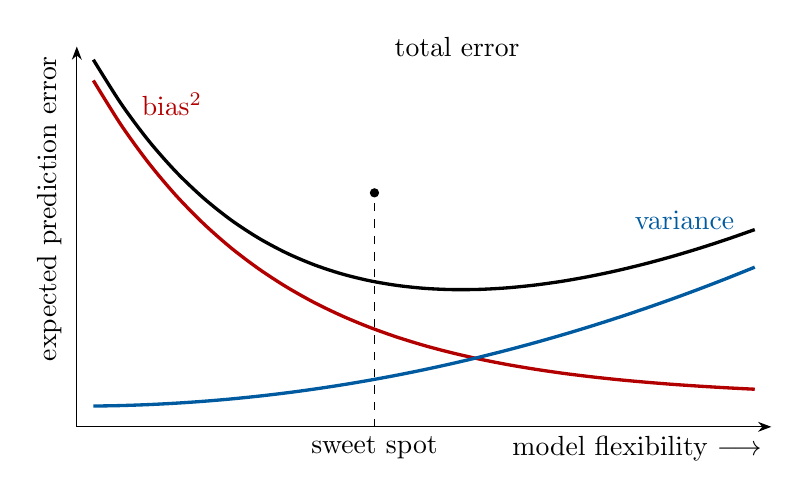
\begin{tikzpicture}[scale=1.05, >=Stealth]
  \draw[->] (0,0) -- (8.4,0) node[below left] {model flexibility $\longrightarrow$};
  \draw[->] (0,0) -- (0,4.6) node[rotate=90, above, anchor=south east, yshift=2pt] {expected prediction error};
  % curves
  \draw[very thick, color=red!70!black, domain=0.2:8.2, smooth] plot (\x, {4.2*exp(-0.45*\x) + 0.35});
  \node[color=red!70!black] at (1.15,3.9) {bias$^2$};
  \draw[very thick, color=accent, domain=0.2:8.2, smooth] plot (\x, {0.25 + 0.05*\x^2/2});
  \node[color=accent] at (7.35,2.5) {variance};
  \draw[very thick, domain=0.2:8.2, smooth] plot (\x, {4.2*exp(-0.45*\x) + 0.35 + 0.25 + 0.05*\x^2/2});
  \node at (4.6,4.6) {total error};
  \draw[dashed] (3.6,0) -- (3.6,2.83);
  \fill[black] (3.6,2.83) circle (1.6pt);
  \node[below] at (3.6,0) {sweet spot};
\end{tikzpicture}
\caption{The bias--variance trade-off. As flexibility grows, squared bias falls fast while variance rises slowly at first, then explosively; their sum has a minimum. Regularization slides a model along this curve by tuning its rigidity.}
\label{fig:ucurve}
\end{figure}

\subsection{Ridge regression: shrinkage with a closed form}

OLS minimizes $\norm{\y - \X\bbeta}^2$. \textbf{Ridge regression} adds a quadratic penalty on the coefficients:
\begin{equation}\label{eq:ridge}
  \bhat^{\mathrm{ridge}} = \arg\min_{\bbeta} \; \norm{\y - \X\bbeta}^2 + \lambda \norm{\bbeta}^2,
  \qquad \lambda \geq 0.
\end{equation}
The penalty shrinks coefficients toward zero; $\lambda$ controls the rigidity. Setting the gradient to zero (Exercise~\ref{ex:ridge}) gives the closed form
\begin{equation}\label{eq:ridge-sol}
  \bhat^{\mathrm{ridge}} = (\X^\top \X + \lambda \bm{I})^{-1} \X^\top \y.
\end{equation}
Three observations, in increasing depth:

\begin{enumerate}[label=(\arabic*)]
  \item \textbf{Numerics}: even when $\X^\top\X$ is singular, $\X^\top\X + \lambda\bm{I}$ is positive definite for any $\lambda > 0$ — ridge \emph{always} has a unique solution. Chapter~\ref{sec:ls}'s numerical trick is Chapter~\ref{sec:bias-variance}'s statistical idea.
  \item \textbf{Geometry}: \eqref{eq:ridge} is a constrained problem — minimize $\norm{\y-\X\bbeta}^2$ subject to $\norm{\bbeta}^2 \leq c$ — whose Lagrangian is \eqref{eq:ridge}. In parameter space, the elliptical contours of the loss meet the ball of radius $\sqrt{c}$; the contact point is interior, biased, and stabler. Correlated features share the coefficient budget instead of fighting over it (Section~\ref{sec:geometry}).
  \item \textbf{Statistics}: with the singular value decomposition $\X = \bm{U}\bm{D}\bm{V}^\top$,
  \[
    \bhat^{\mathrm{ridge}} = \bm{V} \, \mathrm{diag}\!\left(\frac{d_j}{d_j^2 + \lambda}\right) \bm{U}^\top \y,
    \qquad
    \bhat^{\mathrm{OLS}} = \bm{V} \, \mathrm{diag}\!\left(\frac{1}{d_j}\right) \bm{U}^\top \y,
  \]
  where $d_j$ are the singular values. Ridge replaces each fragile factor $1/d_j$ by $d_j/(d_j^2 + \lambda) < 1/d_j$: \emph{it tames exactly the small-$d_j$ (ill-conditioned, high-variance) directions that OLS amplifies}. Viewed through the hat matrix, ridge shrinks the singular values of the projection from $1$ toward $0$; the effective degrees of freedom, $\sum_j d_j^2/(d_j^2 + \lambda) < p+1$, shrink continuously with $\lambda$.
\end{enumerate}

\subsection{Mean-squared-error optimality of shrinkage}

Ridge is biased — so why can it beat BLUE? Compute its MSE in the orthogonal-design case $\X^\top\X = \bm{I}$ (to see the structure without clutter), where
\[
  \bhat^{\mathrm{ridge}}_j = \frac{1}{1+\lambda}\, \hat{\beta}_j^{\mathrm{OLS}}.
\]
Then $\bias_j = -\frac{\lambda}{1+\lambda}\beta_j$ and $\Var_j = \frac{\sigma^2}{(1+\lambda)^2}$, so
\[
  \MSE_j(\lambda) = \frac{\lambda^2 \beta_j^2 + \sigma^2}{(1+\lambda)^2}.
\]
Differentiate at $\lambda = 0$: the MSE \emph{decreases} for any small $\lambda > 0$ whenever $\beta_j^2 < \sigma^2$ — i.e., \emph{shrinking a weak signal beats estimating it honestly}. There exists $\lambda^\star > 0$ with $\MSE(\lambda^\star) < \MSE(0) = \MSE(\mathrm{OLS})$ for every $\bbeta$. This is the regression shadow of Stein's paradox: the unbiased estimator is inadmissible; a little bias buys a better estimator, for every parameter value simultaneously. Gauss--Markov does not contradict this — it simply refuses to enter the biased class where the improvement lives.

\subsection{Lasso and sparsity: a different penalty, a different bet}

Ridge penalizes the \emph{squared} norm; the \textbf{lasso} penalizes the \emph{absolute} norm:
\begin{equation}\label{eq:lasso}
  \bhat^{\mathrm{lasso}} = \arg\min_{\bbeta} \; \tfrac{1}{2}\norm{\y - \X\bbeta}^2 + \lambda \norm{\bbeta}_1.
\end{equation}
Same bias--variance principle, different geometry: the $\ell_1$ constraint region is a diamond with corners on the coordinate axes, and minima tend to occur \emph{at the corners} — i.e., with some coefficients \emph{exactly zero}. Lasso does variable selection automatically. The price: no closed form, and (in general) biased even for large signals; the gain: an interpretable sparse model, and (under ``irrepresentability'' conditions on $\X$) consistent selection of the true support as $n \to \infty$. Ridge bets all coefficients are small; lasso bets most are zero. Which bet wins is a property of the world, not of the math — and cross-validation is the honest way to find out.

\subsection{Choosing $\lambda$: cross-validation, honestly done}

Regularization converts one model into a one-parameter family indexed by $\lambda$. The bias--variance picture says the best $\lambda$ minimizes \emph{expected} prediction error, which we cannot compute — but we can estimate it:

\begin{enumerate}[label=(\alph*)]
  \item Split the data into $K$ folds. For each fold, fit on the other $K-1$ and evaluate the held-out error.
  \item Average the $K$ held-out errors: the cross-validation estimate of prediction error at that $\lambda$.
  \item Pick $\hat{\lambda}$ minimizing the curve; refit on all data; report honest uncertainty (one standard error up the curve is a fine, slightly more parsimonious choice).
\end{enumerate}

The logic is bias--variance again: the training error is a badly biased estimate of prediction error (it rewards overfitting — flexibility in Figure~\ref{fig:ucurve}), while a fresh test set is unbiased but expensive; cross-validation is the practical compromise. Every claim in this chapter about choosing flexibility is operationalized by this loop.

\begin{keybox}[Chapter verdict]
Squared error decomposes into bias and variance; unbiasedness is not the goal, \emph{MSE} is. Shrinkage estimators (ridge, lasso) deliberately incur bias to cut variance, taming the exact ill-conditioned directions OLS amplifies. The tuning parameter selects a point on the bias--variance curve, and cross-validation estimates that point from data. Modern machine learning is, to a first approximation, this one idea scaled up.
\end{keybox}

% Chapter 8
\section[Beyond Straight Lines: Features, Kernels, and Foundations]{Beyond Straight Lines: Features, Kernels, and the Foundation of Everything Else}\label{sec:beyond}

We have kept one promise silently: that the model be linear in $\bbeta$. This chapter cashes in that promise. It shows (i) how ``linear'' quietly becomes ``arbitrarily flexible'' through feature engineering, (ii) how the kernel trick pushes this to infinity, and (iii) why linear regression is the load-bearing element beneath most of the models that displaced it in the headlines.

\subsection{Nonlinear relationships, linear machinery}

Recall the remark in Chapter~\ref{sec:intro}: linearity is required in the \emph{parameters}, not the raw inputs. Given any functions $\phi_1, \dots, \phi_m$ of the raw features — polynomials $\phi_j(x) = x^j$, splines, sinusoids, interactions $x_1 x_2$, indicator functions — define the \emph{basis-expanded design matrix} $\bm{\Phi}$ with rows $(\phi_1(\x_i), \dots, \phi_m(\x_i))$ and fit
\[
  y_i = \sum_{j=1}^m \beta_j \phi_j(\x_i) + \varepsilon_i
  \quad\Longleftrightarrow\quad
  \bhat = (\bm{\Phi}^\top \bm{\Phi})^{-1} \bm{\Phi}^\top \y .
\]
\emph{Every theorem of Chapters \ref{sec:ls}--\ref{sec:probability} applies verbatim}, with $\bm{\Phi}$ in place of $\X$: OLS is BLUE, the $t$- and $F$-tables are exact under Gaussian errors, and ridge regularizes the expanded basis. Taylor's theorem guarantees that smooth functions are locally well approximated by polynomials; splines piece that locality together. ``Why linear regression'' is not ``why draw straight lines'' — it is ``why solve one exactly-solvable convex problem after a wise change of coordinates.''

The one new danger is the bias--variance curve of Chapter~\ref{sec:bias-variance} tilting: with $m$ large relative to $n$, $\bm{\Phi}^\top\bm{\Phi}$ becomes ill-conditioned and variance explodes — which is precisely when ridge (or lasso) stops being optional.

\subsection{The kernel view: infinite features, finite computation}

Here is one of the most beautiful facts in machine learning. Every appearance of the data in the normal equations is through the Gram matrix $\bm{\Phi}\bm{\Phi}^\top$ (or $\bm{\Phi}^\top\bm{\Phi}$). Its entries are inner products:
\[
  [\bm{\Phi}\bm{\Phi}^\top]_{ij} = \sum_{k=1}^m \phi_k(\x_i)\, \phi_k(\x_j) =: K(\x_i, \x_j),
\]
the \emph{kernel} of the basis. For many bases — polynomials of all degrees, radial Gaussians — the function $K(\x, \x')$ has a closed form even though the basis itself is infinite-dimensional. \textbf{Kernel ridge regression} writes the solution entirely in terms of $K$:
\[
  \hat{f}(\x) = \bm{k}(\x)^\top (\bm{K} + \lambda \bm{I})^{-1} \y,
  \qquad
  K_{ij} = K(\x_i, \x_j), \;\; \bm{k}(\x) = (K(\x, \x_1), \dots, K(\x, \x_n))^\top,
\]
an $n \times n$ linear system regardless of the (possibly infinite) number of features. Linear regression on an infinite-dimensional basis is not a slogan; it is a matrix inversion. Gaussian-process regression is exactly this object dressed in probabilistic language. The lesson generalizes: \emph{methods are often separable from representations}, and the linear algebra travels better than the features.

\subsection{Logistic regression: the same geometry, a different noise model}

For binary outcomes $y_i \in \{0, 1\}$ a line predicting raw probabilities is wrong — predictions can leave $[0,1]$. The \textbf{generalized linear model} (GLM) repairs this with a link function:
\[
  \Pr(y_i = 1 \mid \x_i) = g^{-1}(\x_i^\top \bbeta), \qquad g(p) = \log \frac{p}{1-p} \;(\text{logit link}).
\]
Fitting is no longer one matrix inversion — the likelihood is not quadratic — but the \emph{iteratively reweighted least squares} (IRLS) algorithm reveals the lineage: each iteration linearizes the problem around the current fit and solves a \emph{weighted least squares} step (Chapter~\ref{sec:gauss-markov}'s GLS). Logistic regression \emph{is} linear regression, iterated, with weights and a squashing nonlinearity. The geometry (projection onto a tangent space), the theory (asymptotic normality of the MLE), and the diagnostics all inherit from the linear model.

\subsection{Neural networks: stacked, re-fit, regularized regressions}

A one-hidden-layer network with linear output is
\[
  f(\x) = \sum_{k=1}^h w_k \, \sigma(\bm{a}_k^\top \x + b_k) + c,
\]
where $\sigma$ is a nonlinearity (ReLU, sigmoid). Each hidden unit computes a \emph{learned feature} $\sigma(\bm{a}_k^\top \x + b_k)$ — basis functions $\phi_k$ whose shapes are themselves fit from data, instead of chosen by the analyst — and the output layer is literally a linear regression on those features. Training alternates: fix features, solve (regularized) linear least squares; then adjust features by gradient descent. Deep learning, from this vantage, is \emph{representation learning glued to linear regression}, with all the old themes intact: the loss is still (often) squared error, overfitting is still the bias--variance trade-off, and the output layer of every regression network is the formula \eqref{eq:ridge-sol} wearing a GPU.

\subsection{Why this chapter matters for practice}

The pragmatic upshot for someone building models today:

\begin{itemize}
  \item \textbf{Start linear.} Fit OLS on sensibly engineered features first. It is instant, interpretable, honest about its uncertainty, and provides the baseline every fancier model must beat — if a gradient-boosted ensemble cannot beat a well-specified linear model on validation data, ship the linear model.
  \item \textbf{Linearity is a coordinate choice.} Before blaming the model for underfitting, blame the coordinates: logs, interactions, splines, and domain transforms move most ``nonlinear'' problems back into the exactly-solvable regime.
  \item \textbf{The theorems travel.} BLUE, the $t$-table, shrinkage, and cross-validation recur, appropriately modified, in nearly every classical model. Learning them once, properly, in the linear case is the highest-leverage hour in applied statistics.
\end{itemize}

\begin{keybox}[Chapter verdict]
``Linear'' never meant ``simple.'' Linear regression plus features equals nonlinear regression with exact solutions and honest inference; plus kernels equals infinite flexibility in $n \times n$ algebra; iterated and squashed equals logistic regression; stacked and gradient-trained equals neural networks. The most modern models are best understood as answers to the question this tutorial started with: why linear regression?
\end{keybox}

% Chapter 9
\section{When the Assumptions Break: A Field Guide to Failure}\label{sec:practice}

Every theorem in this tutorial has hypotheses. Mature use of linear regression means knowing which hypothesis fails, what symptom it produces, and what the repair costs. This chapter is the diagnostic manual, organized by assumption.

\subsection{Linearity (A1): the model is wrong}

\textbf{Symptoms.} Residuals show structure: curvature in residual-vs-fitted plots, systematic patterns against individual predictors.

\textbf{Consequences.} Bias in everything — coefficients estimate a misspecified average effect; predictions are systematically wrong where curvature lives.

\textbf{Repairs.} Feature engineering (Chapter~\ref{sec:beyond}): polynomial or spline terms, log transforms, interactions. The RESET test and added-variable plots help locate the misspecification. Note the epistemological point: OLS under misspecification still converges to the \emph{best linear predictor} — the linear projection of the truth — which is sometimes all an applied question needs, and honest reporting says so.

\subsection{Full rank (A2): multicollinearity}

\textbf{Symptoms.} Huge standard errors, unstable coefficient signs across resamples, individual $t$-tests insignificant while the overall $F$ is overwhelming, variance inflation factors $\mathrm{VIF}_j = 1/(1 - R_j^2)$ large (say $> 10$).

\textbf{Consequences.} $\mathcal{C}(\X)$ is nearly degenerate (Chapter~\ref{sec:geometry}): predictions at observed $\x$ are fine, but coefficient interpretations and extrapolation collapse. The information to separate correlated predictors is simply absent from the data.

\textbf{Repairs.} Drop or combine redundant features, center and orthogonalize, or — most honestly — switch to ridge regression and interpret the shrunken coefficients as effects ``adjusted for the correlation structure,'' not as isolated causal effects.

\subsection{Homoscedasticity and uncorrelatedness (A3): the variance structure}

\textbf{Heteroscedasticity.} Symptoms: fan-shaped residual plots. Consequences: OLS stays unbiased and consistent, but it is no longer efficient (GLS beats it — Chapter~\ref{sec:gauss-markov}); the immediate practical damage is wrong standard errors, i.e.\ wrong tests and intervals, even though $\bhat$ itself is consistent. Two repairs: (i) \emph{heteroscedasticity-consistent} (Huber--White, ``sandwich'') standard errors, which correct inference without touching the estimator; (ii) GLS with a variance model $\sigma_i^2 = h(\x_i)$.

\textbf{Correlated errors.} In time series and grouped data, $\Cov(\varepsilon_i, \varepsilon_j) \neq 0$ — e.g.\ autocorrelation or cluster dependence. Symptoms: residuals autocorrelated (Durbin--Watson statistic far from 2); consequences: $\hat\sigma^2$ too small, standard errors too small, $t$-statistics far too optimistic, nonsense ``significance.'' Repairs: cluster-robust or Newey--West standard errors; GLS with an autocorrelation model; or mixed models that model the correlation explicitly.

\subsection{Normality (A4): tails and outliers}

\textbf{Symptoms.} Heavy-tailed residuals, a few points with enormous residuals or leverage ($H_{ii}$ near 1), influence statistics (Cook's distance) flagging observations that move coefficients more than the rest of the data combined.

\textbf{Consequences.} With large $n$, CLT (Chapter~\ref{sec:probability}) protects the tests; with small $n$ or severe contamination, inference can be badly wrong, and \emph{estimates} can be dragged off by outliers regardless of $n$.

\textbf{Repairs.} Diagnose with leverage/residual/influence plots (the three measure distinct pathologies: unusual $\x$, large $e$, and large effect on $\bhat$, respectively); use robust losses (Chapter~\ref{sec:why-squared}); use quantile regression if the question concerns medians; never delete ``ugly'' points silently — report sensitivity with and without them (the user's own taste: surface weaknesses honestly, disclose rather than hide).

\subsection{$n$ versus $p$: the modern regime}

Classical theory assumed $n \gg p$; modern data often has $p \geq n$ or $p \gg n$. Then:
\begin{itemize}
  \item $\X^\top\X$ is singular — OLS is not even defined without regularization; ridge/lasso are not enhancements but necessities (Chapter~\ref{sec:bias-variance});
  \item the classical consistency story must be replaced by sparse-recovery theory: under conditions on $\X$ (restricted eigenvalues) and true sparsity, lasso recovers support and $\ell_2$ error $\asymp \sqrt{s \log p / n}$;
  \item honest error estimation requires out-of-sample evaluation — with $p$ comparable to $n$, in-sample $R^2$ is close to meaningless.
\end{itemize}

\subsection{Association is not causation — the assumption nobody writes down}

The linear model estimates conditional associations. Interpreting a coefficient as a causal effect requires an identification strategy (randomization, instrumental variables, difference-in-differences, or unverifiable untestable assumptions like ``no unmeasured confounding''). The machinery of this tutorial says nothing about causality, and no amount of $t$-statistics repairs a broken identification strategy. Say this to yourself every time you open \texttt{lm()}.

\begin{keybox}[The diagnostic loop]
Plot first, test second, repair third, disclose always: (1) residuals vs.\ fitted (linearity, heteroscedasticity); (2) leverage, residual, influence (outliers); (3) Durbin--Watson or cluster structure (correlation); (4) VIF (collinearity); (5) sample size vs.\ dimension (do you even need regularization). Every failure has a named repair that is a modification of OLS — which is the final, practical answer to why linear regression: it is the hub from which all repairs are one spoke away.
\end{keybox}

% Chapter 10
\section{Epilogue: So, Why Linear Regression?}\label{sec:epilogue}

We set out to answer one question. The answer turned out to be seven answers, each a different lens on the same object.

\subsection{The seven answers, collected}

\begin{enumerate}[label=\textbf{\arabic*.}]
  \item \textbf{Because it is exactly solvable.} Squared error turns estimation into a convex quadratic problem with a unique, closed-form, computable-in-milliseconds answer (Chapter~\ref{sec:ls}). No initialization, no local minima, no hyperparameters to speak of.
  \item \textbf{Because squared error is principled, not habitual.} It is the MLE under Gaussian noise, the partner of the maximum-entropy error model, and uniquely tractable; and its known weakness (outliers) has named, classical repairs (Chapter~\ref{sec:why-squared}).
  \item \textbf{Because it is the right projection.} Geometrically, OLS is the orthogonal projection of data onto the model's subspace; the normal equations, the hat matrix, $R^2$, and degrees of freedom are all one picture (Chapter~\ref{sec:geometry}).
  \item \textbf{Because it is provably optimal in its class.} Gauss--Markov: under correct specification, full rank, and homoscedastic uncorrelated errors, no linear unbiased estimator beats it — with zero distributional assumptions (Chapter~\ref{sec:gauss-markov}).
  \item \textbf{Because it supports exact inference.} Add Gaussian errors and the whole apparatus of $t$-, $\chi^2$-, and $F$-distributions follows from one repeated argument about projections of Gaussian noise; remove Gaussianity and the CLT restores it asymptotically (Chapter~\ref{sec:probability}).
  \item \textbf{Because it knows its own limits.} The bias--variance decomposition tells you exactly what OLS's unbiasedness costs, and ridge/lasso/cross-validation are the controlled repairs — the same mathematics that underlies modern machine learning (Chapter~\ref{sec:bias-variance}).
  \item \textbf{Because everything else is built on it.} Feature expansion, kernels, GLMs, IRLS, and the output layer of neural networks are all linear regression, iterated or extended (Chapter~\ref{sec:beyond}).
\end{enumerate}

\subsection{The deeper reason}

Strip away the theorems and one fact remains: the conditional mean $\E[y \mid \x]$ is \emph{the} function that minimizes expected squared prediction error, and the linear model is its simplest honest approximation — two parameters stand between you and a principled answer, interpretable, uncertainty-quantified, falsifiable. Every model in statistics and machine learning is, at bottom, an answer to the same question with different machinery for approximating that conditional mean. Linear regression is the baseline against which all of them are measured, the exact special case in which every quantity can be derived and every assumption audited, and the hub to which every repair routes back.

Legendre published least squares in 1805 to fit orbits from noisy asteroid observations. Two hundred and twenty years later, the same formula fits neural network output layers, genome-wide association studies, and econometric policy evaluation. Anything that survives that much change is not a technique — it is a theorem about how data meets models. That is why linear regression.

\vspace{1.5em}
\begin{center}
\itshape
Fit the line. Audit the assumptions. \\
Disclose the weaknesses. Then — and only then — reach for something fancier.
\end{center}


\appendix
% Appendix A
\section{Linear Algebra Facts Used in This Tutorial}\label{app:linalg}

Everything below is standard; proofs are sketched where they clarify.

\subsection{Notation}

Matrices $\bm{A}, \bm{B}, \dots$ are uppercase bold; vectors lowercase bold; scalars plain. $\bm{A}^\top$ = transpose; $\bm{A}^{-1}$ = inverse (when it exists); $\bm{A}^{+}$ = Moore--Penrose pseudoinverse. $\bm{I}_n$ = $n \times n$ identity. $\norm{\bm{v}} = \sqrt{\bm{v}^\top \bm{v}}$ = Euclidean norm; $\bm{u} \perp \bm{v}$ means $\bm{u}^\top \bm{v} = 0$.

\subsection{Matrix multiplication: two readings}

The product $\bm{C} = \bm{A}\bm{B}$ can be read \emph{by entries} ($C_{ik} = \sum_j A_{ij} B_{jk}$) or \emph{by columns}: column $k$ of $\bm{C}$ is $\bm{A}$ times column $k$ of $\bm{B}$ — a linear combination of $\bm{A}$'s columns. The second reading drives this tutorial: $\X \bbeta$ is the linear combination of predictors with weights $\bbeta$, and $\mathcal{C}(\X)$ is the set of all such combinations.

\subsection{Transpose rules}

$(\bm{A}\bm{B})^\top = \bm{B}^\top \bm{A}^\top$; $(\bm{A}^\top)^\top = \bm{A}$; a scalar satisfies $s^\top = s$, hence $\bm{u}^\top \bm{v} = \bm{v}^\top \bm{u}$. Symmetric matrices satisfy $\bm{A}^\top = \bm{A}$; $\X^\top\X$ and projection matrices are always symmetric.

\subsection{Positive (semi)definiteness}

A symmetric $\bm{A}$ is \textbf{positive semidefinite} ($\bm{A} \succeq \zero$) if $\bm{v}^\top \bm{A} \bm{v} \geq 0$ for all $\bm{v}$; \textbf{positive definite} ($\bm{A} \succ \zero$) if strict for $\bm{v} \neq \zero$. Facts used:
\begin{itemize}
  \item Gram matrices are PSD: $(\X^\top\X) \succeq \zero$ since $\bm{v}^\top \X^\top \X \bm{v} = \norm{\X\bm{v}}^2 \geq 0$; and $\succ \zero$ iff $\X$ has trivial null space (full column rank).
  \item PSD matrices have real nonnegative eigenvalues and orthonormal eigenvectors; PD matrices have positive eigenvalues and are invertible.
  \item A sum of PSD matrices is PSD; adding $\lambda \bm{I}$ ($\lambda > 0$) makes any symmetric matrix PD — this is why ridge always has a unique solution.
  \item $\bm{D}\bm{D}^\top \succeq \zero$ for any $\bm{D}$ — used in the Gauss--Markov proof.
\end{itemize}

\subsection{Inverse: existence and the Woodbury-free facts we need}

$\bm{A}$ invertible $\iff$ null space trivial $\iff$ columns linearly independent. Inverse of a product: $(\bm{A}\bm{B})^{-1} = \bm{B}^{-1}\bm{A}^{-1}$. Invertibility is destroyed by \emph{dependent columns} (exact collinearity) and merely \emph{degraded} by nearly dependent ones (ill-conditioning, quantified by the condition number $\kappa(\X^\top\X) = \lambda_{\max}/\lambda_{\min}$).

\subsection{Vector derivatives}

For $\bm{c} \in \R^p$ and symmetric $\bm{A} \in \R^{p \times p}$:
\[
  \nabla_{\bbeta} (\bm{c}^\top \bbeta) = \bm{c},
  \qquad
  \nabla_{\bbeta} (\bbeta^\top \bm{A} \bbeta) = 2 \bm{A} \bbeta,
  \qquad
  \nabla^2_{\bbeta} (\bbeta^\top \bm{A} \bbeta) = 2 \bm{A}.
\]
Applied to $S(\bbeta) = \y^\top\y - 2\bbeta^\top\X^\top\y + \bbeta^\top\X^\top\X\bbeta$, these give gradient $-2\X^\top\y + 2\X^\top\X\bbeta$ and Hessian $2\X^\top\X$ (positive definite under full rank — hence strict convexity).

\subsection{Eigen- and singular value decompositions}

Every symmetric $\bm{A}$ has $\bm{A} = \bm{Q}\bm{\Lambda}\bm{Q}^\top$ with $\bm{Q}$ orthogonal ($\bm{Q}^\top\bm{Q} = \bm{I}$) and $\bm{\Lambda}$ diagonal of eigenvalues — the engine behind Lemma~\ref{lem:trace} and Theorem~\ref{thm:chi2}. Every matrix has an SVD $\X = \bm{U}\bm{D}\bm{V}^\top$ with $\bm{U}, \bm{V}$ orthogonal and $\bm{D} \geq 0$ diagonal (singular values $d_j$; $d_j^2$ = eigenvalues of $\X^\top\X$) — the engine behind ridge's shrinkage factors in Chapter~\ref{sec:bias-variance}.

\subsection{Trace}

$\trace(\bm{A}) = \sum_i A_{ii}$; $\trace(\bm{A}\bm{B}) = \trace(\bm{B}\bm{A})$ (cyclic, when dimensions match). Used for $\trace(\bm{H}) = \trace((\X^\top\X)^{-1}\X^\top\X) = \trace(\bm{I}_{p+1}) = p+1$.

\subsection{Orthogonal projections}

A matrix $\bm{P}$ is an orthogonal projection (onto its range, along the orthogonal complement) iff $\bm{P}^2 = \bm{P}$ (idempotent) and $\bm{P}^\top = \bm{P}$ (symmetric). Then $\norm{\bm{y}}^2 = \norm{\bm{P}\bm{y}}^2 + \norm{(\bm{I}-\bm{P})\bm{y}}^2$ (Pythagoras), and $\rank(\bm{P}) = \trace(\bm{P})$ (Lemma~\ref{lem:trace}). The hat matrix $\bm{H} = \X(\X^\top\X)^{-1}\X^\top$ is the canonical example; $\bm{I} - \bm{H}$ projects onto the residual space.

% Appendix B
\section{Exercises, with Solutions}\label{app:exercises}

Exercises are ordered by chapter. Each solution is a miniature version of an argument in the text — do them with the book closed, then read.

\subsection*{Chapter \ref{sec:ls}}

\begin{exercise}\label{ex:sigma}
Show that $\hat{\sigma}^2 = \norm{\bm{e}}^2/(n-p-1)$ is unbiased for $\sigma^2$ under (A1)--(A3), i.e.\ $\E[\norm{\bm{e}}^2] = (n-p-1)\sigma^2$.
\end{exercise}
\begin{proof}
Write $\bm{e} = (\bm{I} - \bm{H})\y = (\bm{I}-\bm{H})(\X\bbeta + \bm{\varepsilon}) = (\bm{I}-\bm{H})\bm{\varepsilon}$, since $(\bm{I}-\bm{H})\X = \zero$. With $\bm{M} := \bm{I} - \bm{H}$ (symmetric, idempotent):
\[
  \E[\norm{\bm{e}}^2] = \E[\bm{\varepsilon}^\top \bm{M} \bm{\varepsilon}] = \E[\trace(\bm{\varepsilon}^\top \bm{M} \bm{\varepsilon})] = \E[\trace(\bm{M}\bm{\varepsilon}\bm{\varepsilon}^\top)] = \trace\big(\bm{M}\, \E[\bm{\varepsilon}\bm{\varepsilon}^\top]\big) = \sigma^2 \trace(\bm{M}) = \sigma^2 (n - p - 1),
\]
using $\E[\bm{\varepsilon}\bm{\varepsilon}^\top] = \Var(\bm{\varepsilon}) = \sigma^2 \bm{I}$ and Lemma~\ref{lem:trace}. Hence $\E[\hat{\sigma}^2] = \sigma^2$.
\end{proof}

\begin{exercise}\label{ex:means}
In simple regression (one feature), verify directly that the least-squares line passes through $(\bar{x}, \bar{y})$ and that \eqref{eq:slope} satisfies the second normal equation.
\end{exercise}
\begin{proof}
The intercept equation gives $\hat\beta_0 = \bar{y} - \hat\beta_1 \bar{x}$, so the fitted value at $\bar{x}$ is $\hat\beta_0 + \hat\beta_1 \bar{x} = \bar{y}$. For the slope equation, substitute $\hat\beta_0$:
\[
  \sum_i x_i\big( (y_i - \bar{y}) - \hat\beta_1 (x_i - \bar{x}) \big) = \sum_i (x_i - \bar{x})(y_i - \bar{y}) - \hat\beta_1 \sum_i (x_i - \bar{x})^2 = 0,
\]
using $\sum_i (x_i - \bar{x}) = 0$ to replace $x_i$ by $x_i - \bar{x}$, and the definition \eqref{eq:slope} of $\hat\beta_1$.
\end{proof}

\subsection*{Chapter \ref{sec:why-squared}}

\begin{exercise}
Show that minimizing $\sum_i |y_i - \theta|$ over $\theta$ yields the sample median. What goes wrong with the derivative-based approach, and how does subgradient calculus fix it?
\end{exercise}
\begin{proof}
$|e|$ is not differentiable at $e = 0$; its subgradient is $\mathrm{sign}(e)$ for $e \neq 0$ and $[-1, 1]$ at $e = 0$. Zero must lie in the subdifferential of the objective: $0 \in \sum_i \partial|y_i - \theta|$. For $\theta$ not equal to any observation, the sum equals $\#\{y_i > \theta\} - \#\{y_i < \theta\}$, which is zero exactly when $\theta$ has as many observations above as below — the median. Between observations the subgradient is constant, so the objective is piecewise linear and any median attains the minimum.
\end{proof}

\subsection*{Chapter \ref{sec:geometry}}

\begin{exercise}
Prove that for any $\bm{y} \in \R^n$, $\norm{\bm{H}\bm{y}} \leq \norm{\bm{y}}$, with equality iff $\bm{y} \in \mathcal{C}(\X)$. Conclude $0 \leq H_{ii} \leq 1$.
\end{exercise}
\begin{proof}
$\norm{\bm{y}}^2 = \norm{\bm{H}\bm{y}}^2 + \norm{(\bm{I}-\bm{H})\bm{y}}^2 \geq \norm{\bm{H}\bm{y}}^2$ by orthogonality; equality iff $(\bm{I}-\bm{H})\bm{y} = \zero$, i.e.\ $\bm{y} = \bm{H}\bm{y} \in \mathcal{C}(\bm{H}) = \mathcal{C}(\X)$. For the diagonal: $H_{ii} = \bm{e}_i^\top \bm{H}\bm{e}_i = \bm{e}_i^\top \bm{H}^2 \bm{e}_i = \norm{\bm{H}\bm{e}_i}^2 \geq 0$ and $\norm{\bm{H}\bm{e}_i} \leq \norm{\bm{e}_i} = 1$ by the first part (with $\bm{H}\bm{e}_i \in \mathcal{C}(\X)$, so in fact $H_{ii} = \norm{\bm{H}\bm{e}_i}^2 \in [0,1]$).
\end{proof}

\subsection*{Chapter \ref{sec:gauss-markov}}

\begin{exercise}\label{ex:gls}
Let $\Var(\bm{\varepsilon}\mid\X) = \bm{\Sigma}$ with $\bm{\Sigma} \succ \zero$ known. Show that $\bhat_{\mathrm{GLS}} = (\X^\top\bm{\Sigma}^{-1}\X)^{-1}\X^\top\bm{\Sigma}^{-1}\y$ is the BLUE of $\bbeta$ by applying Gauss--Markov in whitened coordinates.
\end{exercise}
\begin{proof}
The symmetric positive definite $\bm{\Sigma}$ has a square root $\bm{\Sigma}^{1/2} \succ \zero$ (eigendecomposition). Multiply the model by $\bm{\Sigma}^{-1/2}$: $\bm{\Sigma}^{-1/2}\y = \bm{\Sigma}^{-1/2}\X \bbeta + \bm{\Sigma}^{-1/2}\bm{\varepsilon}$. The transformed errors have covariance $\bm{\Sigma}^{-1/2}\bm{\Sigma}\bm{\Sigma}^{-1/2} = \bm{I}$: assumptions (A1)--(A3) hold with design $\tilde{\X} = \bm{\Sigma}^{-1/2}\X$. Applying OLS in the new coordinates and multiplying back gives exactly $\bhat_{\mathrm{GLS}}$; Gauss--Markov makes it BLUE for the transformed problem, and linear unbiasedness is preserved under the invertible transformation.
\end{proof}

\subsection*{Chapter \ref{sec:probability}}

\begin{exercise}
Under (A1)--(A4) with $\X^\top\X = n\bm{I}$ (orthonormal design scaled by $n$), give the exact distribution of $\norm{\bhat - \bbeta}^2$ and use it to build a $1-\alpha$ confidence \emph{ellipsoid} for $\bbeta$.
\end{exercise}
\begin{proof}
By Theorem~\ref{thm:dist-bhat}, $\bhat - \bbeta \sim \mathcal{N}(\zero, \sigma^2 (\X^\top\X)^{-1}) = \mathcal{N}(\zero, \tfrac{\sigma^2}{n}\bm{I})$, so
\[
  \frac{n \norm{\bhat - \bbeta}^2}{\sigma^2} = \sum_{j} \frac{n(\hat\beta_j - \beta_j)^2}{\sigma^2} \sim \chi^2_{p+1}.
\]
Replacing $\sigma^2$ by the independent $\hat\sigma^2 \sim \sigma^2 \chi^2_{n-p-1}/(n-p-1)$ (Theorem~\ref{thm:chi2}) and taking the ratio,
\[
  \frac{n \norm{\bhat - \bbeta}^2}{(p+1)\hat\sigma^2} \sim F_{p+1,\, n-p-1}.
\]
Hence $\big\{ \bbeta : \norm{\bhat - \bbeta}^2 \leq \frac{(p+1)\hat\sigma^2}{n} F_{p+1,\,n-p-1,\,1-\alpha} \big\}$ is an exact $1-\alpha$ confidence ellipsoid (a sphere in these coordinates).
\end{proof}

\subsection*{Chapter \ref{sec:bias-variance}}

\begin{exercise}\label{ex:ridge}
Derive the ridge solution \eqref{eq:ridge-sol} from the penalized objective, and prove that the ridge estimator is biased with $\bias = -\lambda(\X^\top\X + \lambda\bm{I})^{-1}\bbeta$.
\end{exercise}
\begin{proof}
The gradient of $\norm{\y - \X\bbeta}^2 + \lambda\norm{\bbeta}^2$ is $-2\X^\top\y + 2\X^\top\X\bbeta + 2\lambda\bbeta$; setting it to zero and noting $\X^\top\X + \lambda\bm{I} \succ \zero$ gives \eqref{eq:ridge-sol}. Substitute the model:
\[
  \E[\bhat^{\mathrm{ridge}}] = (\X^\top\X + \lambda\bm{I})^{-1}\X^\top\X\,\bbeta
  = \bbeta - \lambda(\X^\top\X + \lambda\bm{I})^{-1}\bbeta,
\]
using $(\X^\top\X + \lambda\bm{I})^{-1}(\X^\top\X) = \bm{I} - \lambda(\X^\top\X+\lambda\bm{I})^{-1}$. The bias term vanishes as $\lambda \to 0$ and saturates as $\lambda \to \infty$ (estimator $\to \zero$).
\end{proof}

\begin{exercise}
In the orthogonal-design ridge setting of Section~7.3, find the $\lambda^\star$ minimizing $\MSE_j$ exactly, and the resulting minimum MSE. For which $\beta_j$ is shrinkage useless?
\end{exercise}
\begin{proof}
$\MSE_j(\lambda) = (\lambda^2\beta_j^2 + \sigma^2)/(1+\lambda)^2$. Setting the derivative to zero:
\[
  \frac{d}{d\lambda}\MSE_j = \frac{2\lambda \beta_j^2 (1+\lambda)^2 - (\lambda^2\beta_j^2 + \sigma^2)\,2(1+\lambda)}{(1+\lambda)^4} = 0
  \;\Longrightarrow\; \lambda^\star = \frac{\sigma^2}{\beta_j^2}.
\]
Then $\MSE_j(\lambda^\star) = \frac{\sigma^2 \beta_j^2}{\beta_j^2 + \sigma^2} < \sigma^2 = \MSE_j(0)$ for any $\beta_j \neq \infty$. As $\beta_j^2 \to \infty$, $\lambda^\star \to 0$ and the gain vanishes: shrinkage is useless (though never harmful in this calculation) for very strong signals — bias--variance thinking allocates shrinkage to weak coefficients.
\end{proof}


\end{document}
